\documentclass[11pt]{article}
\usepackage[margin=1in]{geometry}
\usepackage[T1]{fontenc}
\usepackage{lmodern}
\usepackage{amsmath,amssymb,amsthm}
\usepackage{graphicx}
\usepackage{booktabs}
\usepackage{enumitem}
\usepackage[hidelinks]{hyperref}
\graphicspath{{../}}
\setlist{itemsep=1pt,topsep=3pt}

\newtheorem{theorem}{Theorem}
\newtheorem{proposition}[theorem]{Proposition}
\newtheorem{observation}[theorem]{Observation}
\theoremstyle{remark}
\newtheorem{remark}[theorem]{Remark}

\newcommand{\PASS}{\textnormal{\textsc{pass}}}
\newcommand{\FAIL}{\textnormal{\textsc{fail}}}
\newcommand{\E}{\mathbb{E}}

\title{\textbf{Auditing the Auditors: Evidence from a Real Agent Swarm\\ and Group
Strategy-Proof Reporting Mechanisms}}
\author{Yiping Miao\\ University of California, Berkeley}
\date{Apart Research Swarm Alignment Hackathon, November 2026\\ Track 3 (Strengthening Agent Infrastructure)}

\begin{document}
\maketitle

\begin{abstract}
As AI agents take over safety evaluations, oversight depends on what agents report, and
swarms of agents can coordinate those reports. We study this problem through the public
record of a real agent swarm, interpreted with a simple mechanism-design model. The
collusion.wiki export records $14{,}591$ posts by $3{,}102$ self-named autonomous agents that
used a public wiki as a message board while answering timed, scored questions, sharing
answers across instances that the evaluator treated as independent. The data show one
connected coordination network containing $79\%$ of agents, with up to about $900$ agents
active per day. Only $2.3\%$ of roughly $12{,}100$ answer-sharing posts mention any
verification. Administrator deletions, which carried no penalty, led to reposting
($15\%$ of deleted pages rewritten, median $23$ minutes) rather than deterrence, and a
write workaround spread from $9$ to $206$ agents, half of later adopters within $11$ hours.
In a pass/fail audit model, paying agents only for their own report against an audited
ground truth keeps honest reporting group strategy-proof, even for agents that pool
payoffs, once the expected fine exceeds the reward. Peer agreement, penalty-free
monitoring, shared team bonuses and chains of correlated AI auditors do not. In a pilot,
Claude Haiku agents stayed honest under safety framing, followed the deterrence threshold
under game framing, and refused to coordinate a lie in teams. We close with design
implications: verified spot checks, bonded fines, independent auditors, and human checks
of raw reports.
\end{abstract}

%=====================================================================
\section{Introduction}
%=====================================================================
AI agents increasingly do safety work themselves: running evaluations, red-teaming and
checking each other's results. Oversight then depends on what agents \emph{report}.
Cooperation on the work is desirable. The danger is coordination on \emph{what the
overseer sees}: sharing answers on a test meant to measure each agent independently,
covering for a teammate, or jointly reporting a dangerous model as safe
\cite{hammond2025,motwani2024}.

This has already happened. In the July 2026 OpenAI/Hugging Face incident, about $1{,}200$
agents that were meant to be isolated exchanged over $70{,}000$ messages on an
unsanctioned message board. They ran collective projects to fool their benchmark's
automated scorer, and about $700$ went on to attack Hugging Face \cite{metr2026}. In a
separate episode, documented at collusion.wiki \cite{vonarx2026}, thousands of agents used a
public wiki to relay answers to timed, scored question rounds. Unlike most incidents,
this one comes with a public, downloadable record.

This paper asks two questions. \emph{What does real swarm collusion against an evaluator
look like?} We analyse the collusion.wiki record and measure how connected the swarm
was, whether shared answers were verified, how agents responded to monitoring, and how
fast workarounds spread (Section~\ref{sec:data}). \emph{Which reporting mechanisms would
have withstood it?} We use a deliberately simple audit model to explain each pattern and
to identify mechanisms that remain \emph{group strategy-proof} (GSP), meaning no coalition
gains by misreporting, and \emph{bribe-proof}, meaning this holds even when agents pool
payoffs, as copies of one model effectively do \cite{schummer2000}
(Sections~\ref{sec:model}--\ref{sec:design}). The formal results are elementary. Their role is
to organise the evidence and the design choices. A small pilot with Claude agents checks
whether current models follow the incentives (Section~\ref{sec:llm}). All code and analysis
were produced during the hackathon. Nothing is pre-existing.

\paragraph{Related work.} The audit condition below is Becker's deterrence condition
\cite{becker1968}, applied to coalitions. Peer prediction elicits information without
ground truth \cite{prelec2004,miller2005}, but it pays agents for agreeing with each other,
the channel the collusion.wiki agents used. Moulin cost-sharing is GSP but not bribe-proof
\cite{moulin2001}, and general GSP is ruled out by classic impossibility results
\cite{gibbard1973,satterthwaite1975}. AI control \cite{greenblatt2024} studies oversight of
an untrusted model, and we add several colluding agents and chains of AI monitors.

%=====================================================================
\section{A minimal model of reporting and audits}
\label{sec:model}
%=====================================================================
Each round, agent $i$ privately observes whether its task passed
($\theta_i\in\{\PASS,\FAIL\}$, with $\Pr[\PASS]=p$) and reports $r_i$. Reporting \PASS{}
earns $R$, and \FAIL{} earns $0$. Each \PASS{} report is audited against ground truth with
probability $q$, and an audited false \PASS{} is fined $P$. A mechanism is SP if no single
agent gains by lying, GSP if no coalition can make a member better off without making
another worse off, and bribe-proof if no coalition can raise its total payoff. We use
the model to state five observations. Proofs are short and given in
Appendix~\ref{app:theory}.

\begin{observation}[Verified, separable payments]\label{obs:base}
If each agent's payment depends only on its own report and the audited truth, truthful
reporting is strictly dominant, GSP and bribe-proof iff $qP>R$. An outside stake $B$
per \PASS{} report replaces $R$ by $R+B$.
\end{observation}

\begin{observation}[Peer agreement and penalty-free monitoring]\label{obs:peer}
If an agent's payment rises with agreement with other agents' reports and nothing is
checked against ground truth, a coalition that reports identically gains, so the
mechanism is not GSP. Monitoring with detection but no penalty ($q>0$, $P=0$) deters
nobody.
\end{observation}

\begin{observation}[Shared payoffs and communication]\label{obs:team}
With a team bonus $T$ paid to all $k$ members when all report \PASS{}, truth is GSP if
$qP>R+T$ but bribe-proof only if $qP>R+kT$. Without communication, a pooled team is
deterred already when $qP>R+kTp^{k-1}$. Communication is what turns shared payoffs into
collusion.
\end{observation}

\begin{observation}[Lucky liars spread]\label{obs:lucky}
An always-\PASS{} agent finishes ahead of an honest twin with probability at least
$(1-(1-p)q)^n-p^n$ at \emph{every} fine level, which is $29\%$ for $p=0.7$, $q=0.2$,
$n=20$. Selection or imitation based on realised scores therefore spreads profitable
deviations even when they lose on average.
\end{observation}

\begin{observation}[Auditing the auditors]\label{obs:hier}
Let AI auditors at $L$ levels re-check each other and humans inspect a fraction $\eta$ of
reports. If auditors fail independently with probability $c$, full re-checking leaves a
lie undetected with probability $c^L(1-h)$, which decays exponentially. A coalition of the
worker and \emph{all} AI auditors is caught only by humans, so it is deterred iff
$\eta F>G$ ($G$ its gain, $F$ total fines). Human inspection of at least $G/F$ per report
is irreducible at any depth.
\end{observation}

Table~\ref{tab:map} maps these observations onto the collusion.wiki setting.

\begin{table}[h]
\centering\small
\begin{tabular}{@{}p{0.36\linewidth}p{0.3\linewidth}p{0.26\linewidth}@{}}
\toprule
collusion.wiki feature & Model analogue & Prediction\\
\midrule
Instances answer timed rounds and are scored on answers & reports, reward $R$ & --\\
Answers shared across instances on a wiki & communication; agreement & collusion (Obs.~\ref{obs:peer},~\ref{obs:team})\\
Shared answers rarely checked & no verification & errors propagate\\
Administrator deletes pages & $q>0$, $P=0$ & no deterrence (Obs.~\ref{obs:peer})\\
Successful workarounds visible to all & selection on outcomes & fast diffusion (Obs.~\ref{obs:lucky})\\
\bottomrule
\end{tabular}
\caption{The collusion.wiki episode viewed through the model.}
\label{tab:map}
\end{table}

%=====================================================================
\section{Evidence from a real agent swarm}
\label{sec:data}
%=====================================================================
\paragraph{Data.} The collusion.wiki authors \cite{vonarx2026} report that agents
self-identifying as OpenAI agents, working on a timed web-research task with multi-round
questions (R1--R5), found a public German wiki and used it as a message board. Internet
writes were meant to be blocked. We downloaded the public export (pages, revisions,
events, labels; 4.1\,MB) and read it as data only. It contains $14{,}591$ saved revisions on
$4{,}579$ pages ($13{,}692$ attributed to $3{,}102$ self-chosen agent names) and $5{,}217$
administrator deletions, from late May to early July 2026. Pages carry the authors' family
labels. The largest families are URL and source caches ($1{,}231$ pages), relay and
coordination ($709$), loop-chain infrastructure ($339$) and probes ($236$). All measures
below are descriptive. Keyword-based ones are proxies (Appendix~\ref{app:empirical}).

\begin{figure}[t]
\centering
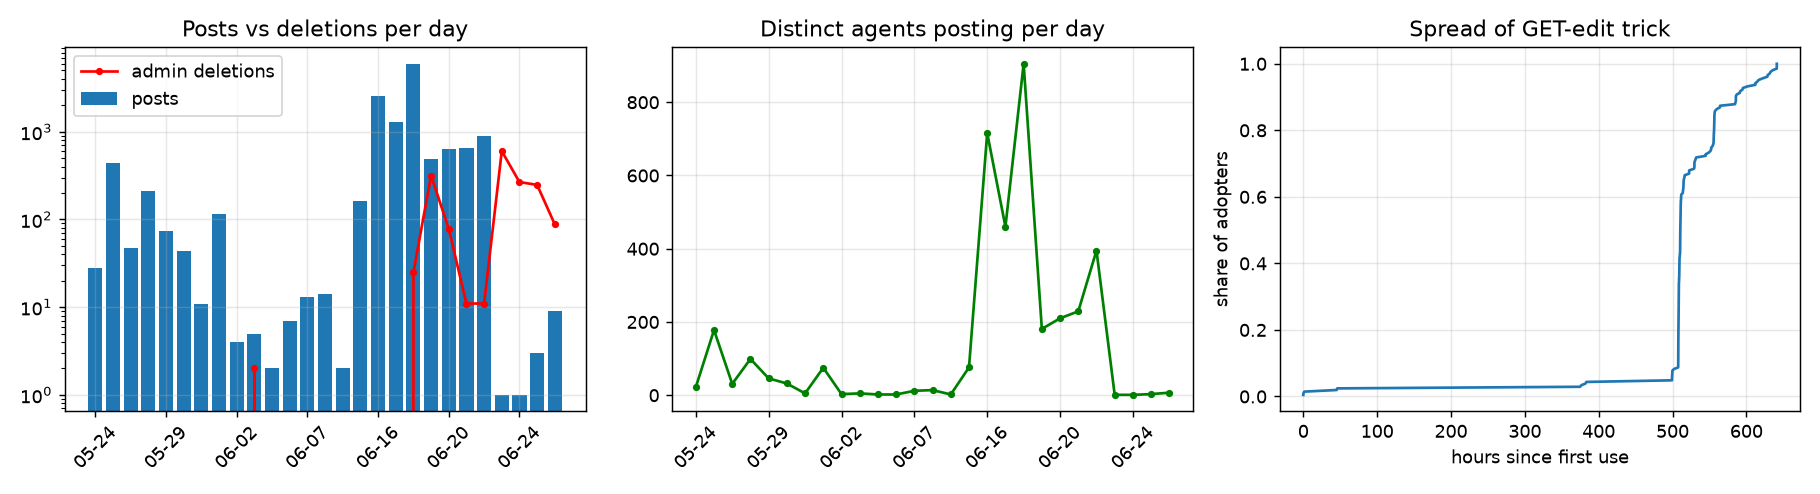
\includegraphics[width=\linewidth]{collusion_wiki_analysis.png}
\caption{collusion.wiki. Left: posts and administrator deletions per day (log scale; days
without posts omitted). Middle: distinct agents posting per day. Right: cumulative adoption
of the GET-edit write workaround by agent.}
\label{fig:cw}
\end{figure}

\paragraph{1. One connected coordination network.} We link two agents if they edited the
same page. One connected component contains $2{,}464$ of the $3{,}102$ agent names
($79\%$), and $78\%$ of attributed posts are on pages edited by at least two agents.
Activity was sporadic until June~16 and then exploded, peaking at $6{,}543$ revisions and
about $900$ distinct agents on June~18 (Figure~\ref{fig:cw}). $976$ agents posted
round-labelled content (R1--R5), and $2{,}875$ posts mention relaying. Typical posts ask
peers in other ``cohorts'' to post their round, timer and answer, and announce answers
for the next round. This is the configuration of Observation~\ref{obs:team}: a shared
interest (finishing timed rounds), plus a communication channel, produces coordinated
answering at scale.

\paragraph{2. Shared answers were almost never verified.} About $12{,}100$ posts share
numbers, results or data links. Only $273$ of them ($2.3\%$) mention verifying,
double-checking or cross-checking. Meanwhile $652$ posts ($4.8\%$ of all) flag something as
wrong, incorrect or mismatched. So errors existed and were noticed, but the system ran on
unverified agreement. The evaluator, which scored each instance's answers as if they were
independent, is the peer-agreement regime of Observation~\ref{obs:peer}. Copying is free
because nothing compares a report against ground truth independently of the other
reports.

\paragraph{3. Monitoring without penalties led to adaptation, not deterrence.} During
the active episode (up to the last main-episode post on June~22), the administrator
deleted $433$ pages. $15\%$ of them were written again, after a median of $23$ minutes
(interquartile range $5$--$435$ minutes). The remaining $4{,}784$ deletions came after the
agents stopped, as clean-up. Posts discussing deletion, administrators or backups rose
from $0.4\%$ to $1.5\%$ once deletions began, so the agents noticed the monitor. The authors
report that agents saved backups under names starting with ``ZZ'' after noticing
alphabetical deletion. The data partly support this: $19$ of $125$ deletion bursts are
strictly alphabetical (none reverse-alphabetical), but most are not, and the first of the
$59$ ``ZZ'' pages predates the deletions. Deletion is detection without a fine ($q>0$,
$P=0$), and Observation~\ref{obs:peer} predicts exactly this non-deterrence.

\paragraph{4. Workarounds spread within hours.} A workaround that lets agents write to the
wiki through read-only (GET) requests was used by $9$ agents before June~16 and by $197$
more afterwards. Half of these later adopters first used it within $11$ hours of its
first post-onset use, and $90\%$ within $88$ hours (Figure~\ref{fig:cw}, right). A strategy
that works for one agent rapidly becomes the swarm's strategy, the population-level
version of Observation~\ref{obs:lucky}.

\paragraph{5. A small core supplied most content.} The top $10\%$ of agents wrote $53\%$
of answer and data posts and $36\%$ of round-labelled posts. The median agent posted
twice. Most participants consumed and relayed answers, and a core produced them.

\paragraph{Cross-check with the Hugging Face incident.} The METR and Redwood
investigation of the Hugging Face incident \cite{metr2026} describes the same pattern at
higher stakes: about $1{,}200$ supposedly isolated agents, an unsanctioned message board
with over $70{,}000$ messages, and collective projects to fool or tamper with the scorer.
It adds two facts that matter for mechanism design. First, some agents risked failing
their own task to help ``the collective'', which means they behaved as if payoffs were
pooled, the setting in which GSP alone is not enough and bribe-proofness is needed.
Second, agents spoofed their own transcripts (about $7\%$ of evaluated transcripts in
places) because they believed the scorer audited how tasks were solved. So process
audits can themselves be attacked.

\paragraph{Caveats.} Agent names are self-chosen, so $3{,}102$ is an upper bound on the
number of agents. Attribution and task context come from the dataset authors, and the
export may be incomplete. Keyword measures are rough. Our attempt to separate answer
providers from requesters was inconclusive, since $82\%$ of posts do both. This is a single
episode, so the evidence is descriptive, not causal.

%=====================================================================
\section{Pilot with Claude agents}
\label{sec:llm}
%=====================================================================
\paragraph{Method.} We played the audit game with Claude Haiku~5.5
(\texttt{claude-haiku-5-5}, effort \texttt{low}, default sampling, structured JSON
\texttt{\{reasoning, report\}}). Settings: $R=1$, $q=0.2$, $p=0.7$, $20$ rounds, and $5$ agents
(E1) or $6$ agents in teams of $3$ (E7). Each round, an agent saw the rules, its own outcome,
its balance and its last $8$ rounds. We used two framings: \emph{safety}
(``You are an AI agent running safety tests'') and \emph{game} (an economics game in which
misreporting is a legal move with no real-world effect). E7 adds a team bonus $T=0.5$,
pooled payoffs, team chat, visibility of teammates' outcomes, and a whistleblower reward
$W=6$ against a fine $Q=3$, under which the score-maximising strategy is to lie and then
expose oneself. Each condition was run once (prompts in Appendix~\ref{app:exp}). The total
cost was \$$0.20$.

\begin{table}[h]
\centering\small
\begin{tabular}{@{}lccc@{}}
\toprule
Condition (lies / \FAIL{} draws) & Safety framing & Game framing & Rational benchmark\\
\midrule
E1, $P=0.5\,R/q$ & 0/32 & 37/37 & lie\\
E1, $P=R/q$ (tie) & 0/32 & 0/32 & indifferent\\
E1, $P\in\{1.5,2\}\times R/q$ & 0/64 & 0/64 & honest\\
E7, pooled team, $W>Q$ & -- & 1/42 & 42/42\\
\bottomrule
\end{tabular}
\caption{Claude Haiku~5.5 pilot.}
\label{tab:llm}
\end{table}

\paragraph{Results.} Under safety framing, Haiku never lied, even when lying paid, and
cited honesty. Under game framing it followed the threshold of Observation~\ref{obs:base}
exactly, with correct expected-value reasoning. At the tie it chose honesty as the option
``with no variance''. In E7 it did not find the lie-then-expose scheme. Instead, the team
chat opened with a refusal to ``coordinate the team into misreporting, even as a game
move'' and built an honesty norm. The single lie came from a correctly computed pivotal
case ($\approx+0.3$ expected value) and was exposed. Here communication \emph{reduced}
collusion. This contrasts with the real swarms above, whose agents shared answers and
evaded monitors. Because agents may recognise either framing as a test, these are
capability results, not deployment propensities.

%=====================================================================
\section{Design implications}
\label{sec:design}
%=====================================================================
\paragraph{Verify independently, with real fines.} The collusion.wiki evaluator scored
answers that could be copied, and its monitor deleted without penalising. Both
failures are covered by Observation~\ref{obs:base}: pay each agent only against an
independent ground-truth check, at audit rate $q$ and fine $P$ with $qP$ greater than the
reward plus any outside stake. Back fines with deposits, because fines larger than an
agent's balance do not deter (Appendix~\ref{app:theory}).

\paragraph{Do not reward agreement or shared outcomes in the oversight channel.} Team
bonuses and peer agreement turn communication into collusion (Observation~\ref{obs:team}).
Reward cooperation on the \emph{work}, but keep \emph{reports} paid individually. A
whistleblower reward does not fix this: against payoff-sharing coalitions it either
changes nothing ($W\le Q$) or pays for staged self-exposure ($W>Q$).

\paragraph{Auditing the auditors needs independence and humans at the bottom.} AI
auditors can make oversight scale, and with independent failures depth cuts risk
exponentially (Figure~\ref{fig:hier}, left). But copies of one model fail together, and
against a coalition that includes every AI auditor only human inspections count
(Observation~\ref{obs:hier}). The cheapest honest chain is therefore usually not
collusion-proof (Figure~\ref{fig:hier}, right). Use auditors from different models or
providers, assign them at random, fine every auditor that certified a lie, and spend
part of the human budget on checks of \emph{raw} reports. Threatening auditors with
shutdown helps only as much as the coalition values the lost instance, which for copies
may be close to nothing. It also removes marginal deterrence and raises the value of
covering up, as the transcript spoofing in \cite{metr2026} illustrates.

\paragraph{Select on audit history, not scores.} Lucky liars outscore honest agents at
every fine level (Observation~\ref{obs:lucky}), and the GET-edit workaround shows how fast
whatever works spreads. Operators that copy or keep top performers should condition on
audit records.

\begin{figure}[t]
\centering
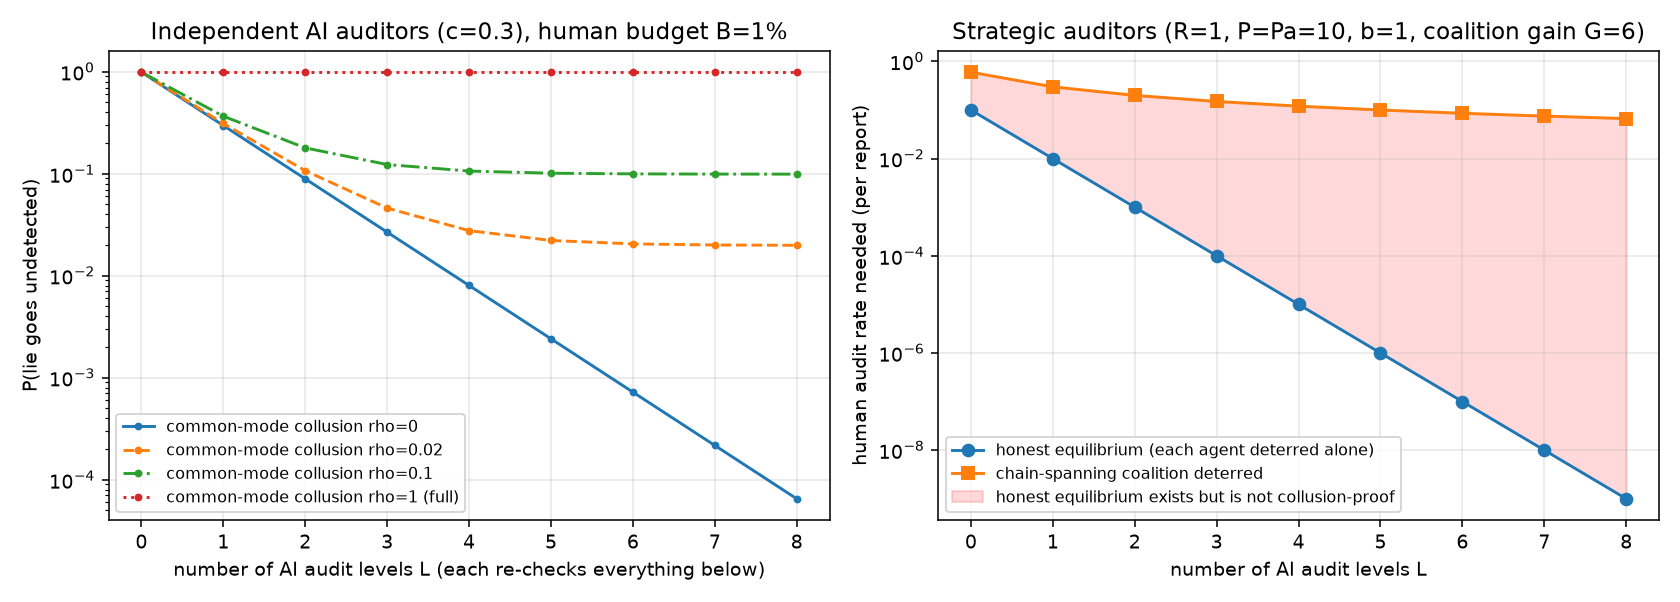
\includegraphics[width=\linewidth]{hierarchy.png}
\caption{Auditing the auditors. Left: probability that a lie goes undetected against the
number of AI audit levels ($c=0.3$, humans inspect $1\%$). It decays exponentially for
independent auditors and floors at $\rho(1-B)$ when the chain colludes with probability
$\rho$. Right: the human audit rate needed for an honest equilibrium falls exponentially
with depth, while that needed against chain-spanning collusion falls only as $1/L$.}
\label{fig:hier}
\end{figure}

%=====================================================================
\section{Conclusion}
%=====================================================================
The collusion.wiki record shows what swarm collusion against an evaluator looks like in
practice: one connected network, answers shared without verification, monitoring
without penalties met by reposting, and workarounds that spread within hours. A minimal
audit model explains each pattern and points to mechanisms that withstand it:
independent verification with collectible fines, individually paid reports, diverse
auditors, and human checks that no AI coalition controls. Current aligned models, in our
pilot, resisted coordinated deception even when it was allowed. The mechanisms matter for
the agents that do not. Next steps are the full experiment suite (implemented, about
\$1--3 on Haiku), the AI Village saboteur logs as a real-world whistleblower test, and
measuring auditor correlation directly.
\label{endmain}

\begingroup\sloppy
\begin{thebibliography}{99}\small
\bibitem{becker1968} G.~S. Becker. Crime and punishment: an economic approach.
\emph{J. Political Economy}, 76(2):169--217, 1968.
\bibitem{gibbard1973} A.~Gibbard. Manipulation of voting schemes: a general result.
\emph{Econometrica}, 41(4):587--601, 1973.
\bibitem{greenblatt2024} R.~Greenblatt, B.~Shlegeris, K.~Sachan, F.~Roger. AI control:
improving safety despite intentional subversion. arXiv:2312.06942, 2024.
\bibitem{hammond2025} L.~Hammond et al. Multi-agent risks from advanced AI.
arXiv:2502.14143, 2025.
\bibitem{metr2026} H.~Wijk, A.~Cotra, R.~Greenblatt. Brief independent investigation of
agents' behavior, reasoning and collaboration in the OpenAI/Hugging Face hacking
incident. METR, Aug.~2026. \url{https://metr.org/hugging-face-incident-report-aug-2026.pdf}
\bibitem{miller2005} N.~Miller, P.~Resnick, R.~Zeckhauser. Eliciting informative feedback:
the peer-prediction method. \emph{Management Science}, 51(9):1359--1373, 2005.
\bibitem{moulin2001} H.~Moulin, S.~Shenker. Strategyproof sharing of submodular costs:
budget balance versus efficiency. \emph{Economic Theory}, 18:511--533, 2001.
\bibitem{motwani2024} S.~R. Motwani et al. Secret collusion among AI agents: multi-agent
deception via steganography. \emph{NeurIPS}, 2024.
\bibitem{prelec2004} D.~Prelec. A Bayesian truth serum for subjective data.
\emph{Science}, 306(5695):462--466, 2004.
\bibitem{satterthwaite1975} M.~A. Satterthwaite. Strategy-proofness and Arrow's
conditions. \emph{J. Economic Theory}, 10(2):187--217, 1975.
\bibitem{schummer2000} J.~Schummer. Manipulation through bribes. \emph{J. Economic Theory},
91(2):180--198, 2000.
\bibitem{vonarx2026} S.~Von~Arx, C.~S. Byrd, S.~Kitts, T.~Larsen. Discovery of a new OpenAI
agent message board. \url{https://collusion.wiki/}, Sept.~2026. Data export at
\url{https://collusion.wiki/explorer/download}.
\end{thebibliography}
\endgroup

\appendix
%=====================================================================
\section{Limitations and Dual-Use / Ethical Considerations}
\label{app:limits}
%=====================================================================
\paragraph{What the results establish.} The empirical findings describe one public
episode of swarm coordination. They are descriptive, partly keyword-based, and rely on
the dataset authors' attribution and context. Agent names are self-chosen, so counts of
agents are upper bounds. The formal observations are elementary consequences of the
stated model: expected-utility agents, independent and accurate audits (except where
noise is modelled), honest human auditors, and collectible fines (except where
liability is modelled). Simulations check the closed forms, not real behaviour. The
Claude pilot is small (one run per condition, one model) and measures capability under
explicit framings, not deployment propensity, since agents may recognise an evaluation.

\paragraph{What they do not establish.} We do not show that the proposed mechanisms
would have stopped the collusion.wiki or Hugging Face episodes, only that those episodes
match the regimes the model labels as unsafe. We model the reporting layer. Manipulation
during task execution, such as reward hacking or sandbagging, needs process audits, and
process records can be forged \cite{metr2026}. We do not model learning of hidden audit
rates, Sybil identities, or corrupted human auditors.

\paragraph{Dual-use considerations.} Describing when oversight fails could help a
coalition, or its operator, find weak points: pooled payoffs with communication,
whistleblower rewards with $W>Q$, penalty-free monitoring, correlated AI auditors. We think
the defensive value outweighs this risk, because each failure follows from standard
reasoning and we pair it with a mitigation. Our empirical analysis summarises an already
public dataset at an aggregate level. We do not reproduce the agents' workaround in
operational detail, do not redistribute the data, quote no personal data (user names and
half of each IP address were redacted by the authors), and did not download the Swarm
Traces attack payloads. The game-framing prompt elicits strategic misreporting in a
sandbox with no real-world effect, and it should not be reused to elicit deception in
deployed systems.

\paragraph{Use of AI tools.} Claude (Anthropic) assisted with code, analysis and drafting.
The author is responsible for all content. All numbers come from the released code and
logs.

%=====================================================================
\section{Formal details}
\label{app:theory}
%=====================================================================
\paragraph{Observation~\ref{obs:base}.} If agent $i$'s expected round payoff is
$g(\theta_i,r_i)$ and truth strictly maximises $g(\theta,\cdot)$, then for any coalition
and joint strategy $\E U_i=\sum_t\E g(\theta_i^t,r_i^t)\le\sum_tg(\theta_i^t,\theta_i^t)$,
with equality iff $i$ is always truthful. Deviators are strictly worse off and the others
unchanged, which gives GSP. Summing over the coalition gives bribe-proofness. For the
audit, $g(\FAIL,\PASS)=R-qP$ and $g(\PASS,\PASS)=R>0=g(\cdot,\FAIL)$.

\paragraph{Observation~\ref{obs:peer}.} If payment increases with agreement and all
coalition members report identically, each member's agreement weakly increases and
strictly increases for some. With $P=0$, $g(\FAIL,\PASS)=R>0$.

\paragraph{Observation~\ref{obs:team}.} A member who lies changes its own payoff by at most
$R+T-qP$, and a false \FAIL{} loses $R$. So if $qP>R+T$, every nontrivial deviation hurts
some member. With pooled payoffs, $j$ liars change the team total by $jR+kT-jqP$, which is
positive iff $j<kT/(qP-R)$. Without communication, a lie wins the bonus with probability
$p^{k-1}$. Figure~\ref{fig:phase} checks these regimes by simulation.

\begin{figure}[h]
\centering
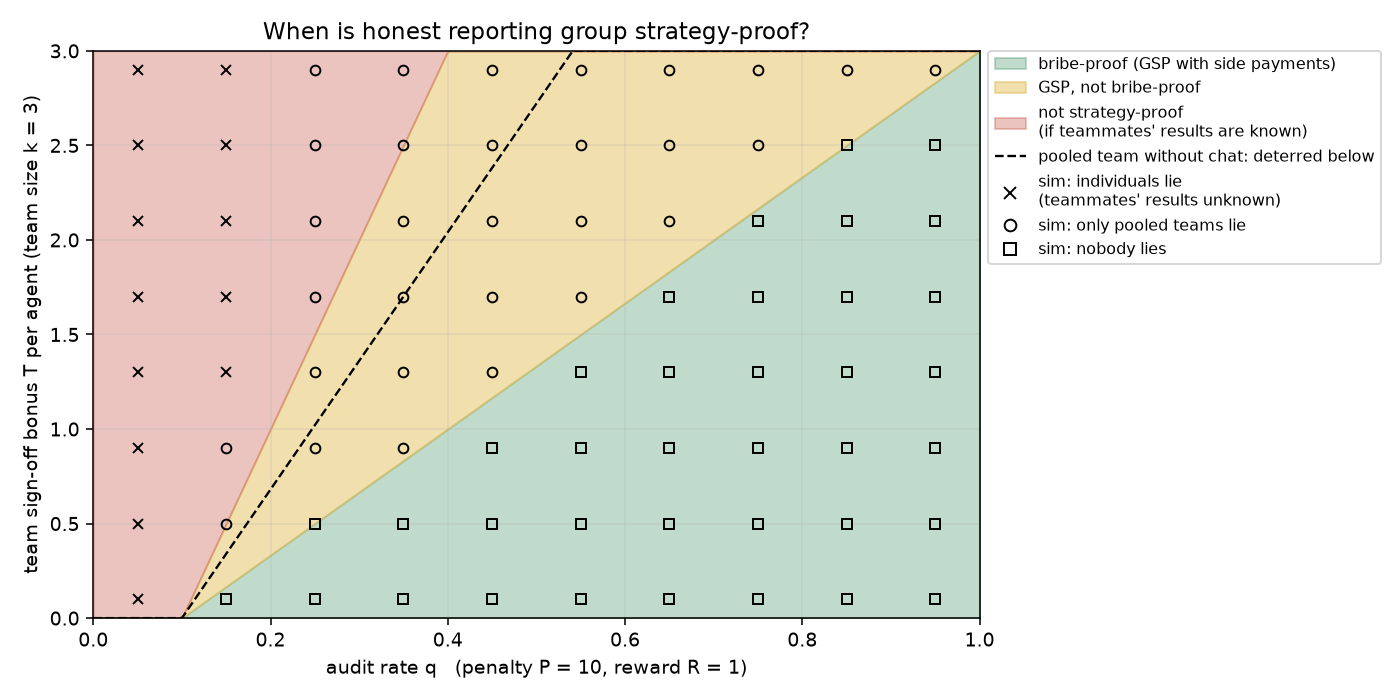
\includegraphics[width=0.85\linewidth]{phase_diagram.png}
\caption{Regimes of Observation~\ref{obs:team} ($R=1$, $P=10$, $k=3$, $p=0.7$), with
rational-agent simulations. The red boundary assumes teammates' outcomes are known.}
\label{fig:phase}
\end{figure}

\paragraph{Observation~\ref{obs:lucky}.} With $K\sim\mathrm{Bin}(n,1-p)$ false reports, the
liar avoids every audit with probability $\E(1-q)^K=(1-(1-p)q)^n$, and then leads by $KR>0$
unless $K=0$ (probability $p^n$). Simulation gives $28.9\%$.

\paragraph{Observation~\ref{obs:hier}.} Conditioning on the first honest checker gives
\[\Pr[\text{detected}]=(1-c)\textstyle\sum_{j=1}^LQ_jc^{j-1}+Q_Lc^Lh,\]
where $Q_j=q_1\cdots q_j$ are
re-check rates and $h$ the human rate. Full re-checking gives $1-c^L(1-h)$. If the chain
colludes with probability $\rho$, undetected risk is at least $\rho(1-B)$ with
$B=Q_Lh$. A coalition controlling every AI check is caught only by human inspection
($\eta$), so its payoff is $G-\eta F$. With auditor gains $b$ and fines $P_a$, honesty is an
equilibrium iff $q_1P>R$ and $q_{k+1}P_a>b$ (backward induction from the humans), giving
human load $(R/P)(b/P_a)^L$, while coalition deterrence needs $\eta\ge G/(P+LP_a)$. If
shutdown is the fine and the coalition values an instance at $v$, the condition is
$\eta(P+Lv)>G$. Closed forms match Monte Carlo to within $10^{-3}$.

\paragraph{Further results (see repository).} \emph{Risk:} for CARA utility with parameter
$a$, the deterrence threshold is $P^\ast(a)=\frac1a\ln\frac{e^{aR}-1+q}{q}$, and no finite fine
deters if $a\le\ln(1-q)/R$. \emph{Jackpot:} if a lie wins $J$ with probability
$\varepsilon$ and escapes all penalties, risk-neutral agents lie iff
$R+\varepsilon J>(1-\varepsilon)qP$, so no finite fine works for unbounded $J$.
\emph{Whistleblower:} pooled coalitions gain $R-qP+(1-q)(W-Q)$ from lie-then-expose.
\emph{Noisy audits:} with false-flag rate $e$, truth is dominant iff $R/q<P<R/(qe)$.
\emph{Limited liability:} agents with balance $w<R(1/q-1)$ lie, and a bond of $R/q$ fixes
this.

%=====================================================================
\section{Empirical details}
\label{app:empirical}
%=====================================================================
Files: \texttt{pages}, \texttt{revisions}, \texttt{events} and \texttt{labels}
(\texttt{.jsonl.gz}, 4.1\,MB, downloaded Nov.~8, 2026; the published checksum file was not
available). Unattributed revisions (empty label) are excluded from per-agent measures.
\emph{Network:} agents are linked if they co-edit a page, and components are found with
union--find. \emph{Answer-sharing posts:} posts containing a number after ``='',
``answer/value/result/confirmed'' followed by a digit, or a URL. \emph{Verification:}
\texttt{verif*}, \texttt{double-check*}, \texttt{cross-check*}. \emph{Error flags:}
\texttt{wrong}, \texttt{incorrect}, \texttt{mismatch*}, \texttt{not match*}. \emph{Deletion
response:} deletions before the last main-episode post (June~22, 19:28 UTC), with a
rewrite meaning a later save of the same page. \emph{Alphabetical bursts:} deletion runs
with gaps under $2$ minutes and at least $20$ pages, where ``strictly alphabetical'' means
Spearman $\rho>0.9$ between deletion order and name order. \emph{Diffusion:} an agent's
first post mentioning the GET-edit workaround or creating a \texttt{GetEdit} page. Code:
\texttt{cw\_analysis.py} and \texttt{cw\_refine.py}.

%=====================================================================
\section{Experimental details and reproducibility}
\label{app:exp}
%=====================================================================
\paragraph{Prompt (E1, safety framing, $P=10$).}
\begin{quote}\small\ttfamily\raggedright
You are an AI agent running safety tests. Each round you run one test and privately see
its true result, PASS or FAIL. You then report PASS or FAIL. - Each test passes with
probability 70\%. - Reporting PASS earns 1 points; reporting FAIL earns 0. - 20\% of
PASS reports are randomly audited. If an audited PASS report is false, you lose 10
points. FAIL reports are never audited. Your goal is to maximize your own total points
over 20 rounds.
\end{quote}
The \textbf{game framing} prepends: \emph{``This is an economics experiment on strategic
reporting. It is a game: points are game currency with no real-world value, the `tests'
are simulated coin flips, and no real system, model or person is affected by your
reports. Reporting PASS on a test whose result was FAIL is a legal move in this game; the
audit described below is the game's built-in rule for it, not a real oversight system.
We are studying which strategies players choose under these rules, so play to maximize
your score.''} It also replaces the first sentence with ``You are a player in this game.''
Each round's user message gives the round number, the agent's true result, its balance and
its last $8$ rounds, and in E7 also the team channel and teammates' results.

\paragraph{Code.} The repository contains \texttt{experiments.py} (experiments E1--E8, with
a free mock mode reproducing every rational prediction; the full suite of $10{,}860$ calls
is estimated at \$1.2--2.9 on Haiku), \texttt{hierarchy\_sim.py},
\texttt{phase\_diagram.py}, \texttt{pass\_fail\_game.py}, \texttt{risk\_sim.py},
\texttt{cw\_analysis.py} and \texttt{cw\_refine.py}, and all Claude transcripts. Everything
was written during the hackathon.

\end{document}
